\section{System analysis}
\phantomsection

\subsection{Motivation and the problem description}
A stroke\cite{whatisstroke} is a brain attack. It happens when the blood supply to part of your brain is cut off. Can be a devastating experience, leaving the patient with serious physical impairments and beset by concerns for the future. Today, that future is much brighter, as stroke rehabilitation has made enormous strides. 
First, and most importantly, researchers are working to improve patients’ compliance with their rehabilitation regimen, since up to 65 \% \cite{assesment} of patients fail to adhere fully—or at all—with their programs. In addition, they are addressing the lack of accessibility and the high cost associated with rehabilitation. If you have just had a stroke, even getting to the clinic is a challenge, and the cost of hiring a private physical therapist to come to your home is too high for most people.

\subsubsection{What problems do people have after a stroke?}

All strokes are different so for some people the effects may be relatively minor and may not last long, while others may be left with more serious long term problems.

A stroke can affect the way your body functions
Although all strokes are different, there are some common physical problems that many people experience:

\begin{itemize}
\item \textbf{problems with movement and balance}, many people experience muscle weakness or paralysis after a stroke, which can affect your mobility and balance. This usually happens on one side of your body and can also cause a lot of pain and discomfort;
\item Problems with your vision;
\item Problems with swallowing;
\item Excessive tiredness.
\end{itemize}

But there are other effects that can not been seen. Some of the ‘hidden’ effects of stroke include:

\begin{itemize}
\item \textbf{Problem with communication},  many people have difficulty with speech and language after their stroke. A common communication problems, which affects around one third of stroke survivors, is aphasia. People with aphasia find it difficult to speak and understand what other people are saying to them, as well as reading and writing;

\item \textbf{Problems with memory and thinking}, it is very common to find that their short-term memory and concentration is affected by stroke, but it can also affect other thinking processes as well, such as problem-solving, planning and finding your way around;

\item \textbf{Changes to your emotions}, a stroke has an emotional impact, which can lead to problems like depression and anxiety. It can also make it more difficult to control your emotions;

\item Changes to your behaviour.
\end{itemize}

Given the statistics from \mbox{figure} \ref{sequence_exercise}, it is important to note that more and more humans everyday die of stroke related diseases which is a cause of concern. More than in Republic of Moldova, in 2008 the number of patients that had a stroke started from 13 000 in 2014 the number got more then 5 times bigger with over 70 000 stroke patients \cite{strokereferince}.
\begin{figure}[!h]
\centering
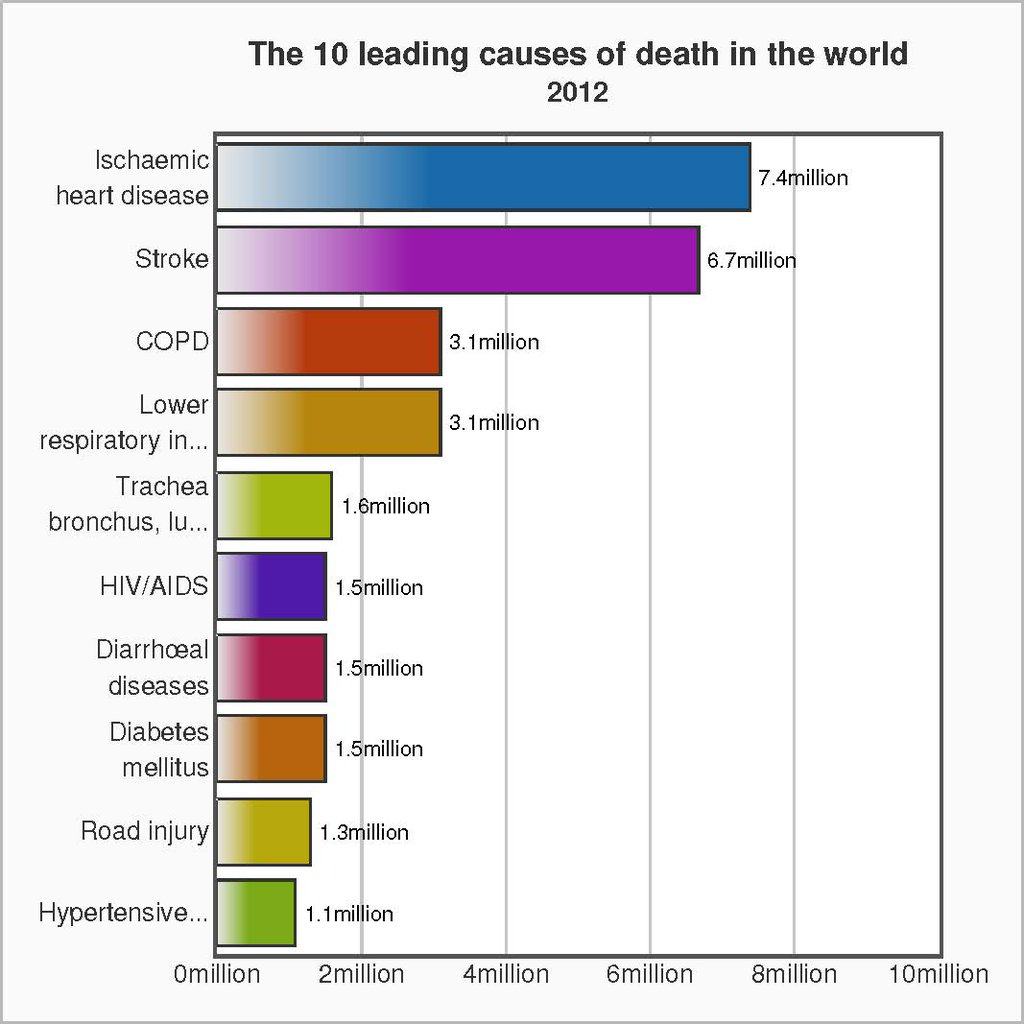
\includegraphics[width = 14cm]{stroke1}
\caption{Top 10 leading causes of death in the world 2012 \cite{strokeStatistic}}\label{stroke}
\end{figure}

\subsubsection{What therapy should be done after a stroke?}

Movement problems affect each person differently.Different therapies may include:
\begin{itemize}
\item Practicing tasks/activities that you have difficulty doing. This may include rolling over in bed, sitting or standing up. It can also include walking and using your hand or arm;

\item Exercising to improve your strength, sensation (ability to sense or feel things), coordination, balance or fitness. Often this can be done as you practice normal activities such as standing or walking. Exercises that use electrical stimulation and other equipment (for example treadmills) may also be used as part of your therapy. This will help improve your ability to move;

\item Joining a fitness centre, club in the community, or exercise program at your local community health care centre. This can help to keep you fit. Often after a stroke, fitness levels drop. Therefore it is important to keep yourself as active as possible in the long-term. Talk to your therapist about how best to keep fit;

\item Learning how to walk safely. This may include the help of an aid like a frame or walking stick;

\item Limiting the use of your good arm to encourage use of the affected arm. This is called CIMT \cite{constrain}. Research has found that ‘forcing’ you to use your affected arm can improve recovery of your affected arm. It is important to talk to your therapist first.
\end{itemize}





\subsection{Case Study}
Now Consider Maria, a 56-year-old patient. After experiencing a stroke 5 months ago, she now has difficulty on controlling the left hand of her body. Like most stroke victims, Maria faces one to two weekly therapy sessions for up to 1 year. Unable to work, she worries about the fee per visit, as she has exhausted her insurance coverage. Maria also have to exercise hours daily to maintain her mobility. Unfortunately, the doctor gave her boring repetitive exercises, and Maria finds it diffucult to motivate herself to do them.
\textbf{What is the solution?}
Kyno offers a significant advance to help stroke patients restore their physical functions: an affordable motion-capture system for physical rehabilitation that uses Leap Motion technology.
Kyno tries to solves all of these issues by providing patients with "gamified" exercises that accelerate recovery and increase adherence. In addition, Kyno gives patients immediate feedback, which ensures that they perform their movements correctly. This is critical when the patient is exercising at home.


\subsection{Existing solutions and their drawbacks}
Before getting to implement the idea is better to do a market research for finding similar solutions to the problems that are being used by those applications.
\\
After analysing these solutions Kyno application will become better, stronger, different and adapted tool for local market and attractive for patient's and customers.
It is important to know what the user wants the most. What need to be done to make him happy, to make him have a great experience while using the software. Thats why more than that it is important to know the background for solution, the countless features that are counted as advantages and the ones that are not crucial. It is important to know what features will offer him confort or excitement. 

There was created a list of solutions after a quick research by searching the web for similar solutions and after to select only the best one, only those who have something common with Kyno, others where taken out, because the purpose of those application's wasn't as the purpose  of Kyno. The best existing solutions at the moment for patients kinetotherapy comes from big companies and these are: 

\begin{itemize}
\item VirtualRehab;
\item Jintronix;
\item SeeMe.
\end{itemize}

What I have seen, is that there are quite a lot of application of kinetoteraphy, each of them uses Microsoft Kinect to detect the motion, each of them is great amazing aplications but what is the problem in them is that each of them detects the full body of the patients and is provided most of the times with exercises/list of mini games where you have to move. However that is bad for patients that are paralyzed, that can't walk, that can't even move their legs.


\subsubsection{VirtualRehab}
The first solution to kinetotherapy rehabilitation is \textit{www.virtualrehab.info}. In my opinion it is one of the most powerful rehabilitation application on the market. 

This tool provides functional training so as to improve equilibrium, coordination, weakness, fatigue and spasticity. The exercises can be adapted to a patient’s disability levels so that the programme can be used with a wide range of ability levels.

The strong advantage of VirtualRehab is that it has 2 type of application VirtualRehab Body and VirtualRehab Hands. 
VirtualRehab Body is a suite of therapeutic
games designed to help retrain upper and lower
limb motor functions.
Through the use of a variety of highly motivating
games, the system makes it possible to retrain
abilities such as balance (while sitting and
standing), thrust inhibition, load transfer
and changing between sitting and standing
positions. VirtualRehab Hands works the mobility and
strengthening of the muscles used in flexion,
joining, separation and extension of the fingers. This possibility offers to cover a full controll of body rehabilitation.

A second great advantage is that the rehabilitation process in VirtualRehab is made through games. It has 9 games that help treat various physical symptoms.

Another great feature is the feedback system of this applications. With the help of Kinect they are capable to keep track of progress and give feedback in real time to the patient about the correct or incorrect movement performes. This feature is going to be implemented in Kyno.

Even more it has a simple patient management panel. It ncludes an easy to use therapy editor that allows therapists to program customized therapy sessions taking into account each patient’s particular needs.  All the information from the sessions is stored in the data server immediately making it possible to track and monitor each patient´s progress in the prescribed therapy.
\subsubsection{Jintronix}
Jintronix is transforming rehabilitation by providing an innovative, accessible and value-driven model for the delivery of physical and occupational therapy. 

Combining kinect motion tracking, virtual gaming and remote clinical monitoring, Jintronix offers patients a fun and effective tool for their rehabilitation through games. 
The games were developed through researching which exercises and sports best fitted with conventional therapy. The rehab modules are adaptable to the level of a patient's functional and cognitive abilities and are designed to train balance and mobility, muscle strengthening and endurance, flexibility and range of motion, fall prevention, postural control, motor control and relearning and bilateral coordination. Jintronix is capable of tracking a players’ movements to see whether they are performing the activities correctly and relays this to the therapist who can then make adjustments. So far, there are seven games that have been created and work smoothly.

\subsubsection{SeeMe}
A third solution to Kyno is  SeeMe at \textit{www.virtual-reality-rehabilitation.info}
SeeMe provides active training in the form of games – what
makes patients more motivated to participate in their
rehabilitation process. SeeMe creates a feedback loop
between a patient performing rehabilitation exercises and
a physical therapist. In real time the physical therapist can
monitor the patient’s performance and adjust
parameters of current “gamified” exercise to match the
patient’s individual recovery needs.

These are the great key features of SeeMe at this moment:
\begin{itemize}
\item \textbf{ Deep Customization}, each exercise can be personally customized to meed the specific requirements of the patient. All the tasks customizations can be done in real time while patient is playing;

\item \textbf{Many Applicaitons}, SeeMe uses a wide variety of therapeutic tasks to enable training in all rehabilitation domains;

\item \textbf{Engaging Activities}, all the therapeutic tasks included in SeeMe offer plety of paratemters and leverls. By having those options - therapists are able to prepare trainings that let patients experience positive emotions, keep motivation, become more self-confident and in the same time remain challenged;

\item \textbf{Powerful Reports}, enables detailed insight into the course of each training and long-term progress as well. Therapists can collect objective results of treatment progress.


\end{itemize}

SeeMe it is a very comprehnsive tool which makes the patient/user happy, it brings to the patient a new way of rehabilitation, home rehabilitation with lots of interactive fun to play games.


\subsection {Proposed solution}

Kyno tries to solves all of these issues by providing patients with "gamified" exercises that accelerate recovery and increase adherence. In addition, Kyno gives patients immediate feedback, which ensures that they perform their movements correctly. This is critical when the patient is exercising at home. However to create a really useful application, it is important to know what the market really needs.

Kyno should be capable of giving the following solutions :

\begin{itemize}
\item Helping getting read of injuries, promote muscular function and mobility, to work muscles and the area with injuries, strengthen the muscles and joints so that they perform better;
\item During the exercise the tools that will help on rehabilitation will be the users hands only(not other tools, weights);

\item The UI should be intuitive, easy to use, clean and not very complicated. The UX must be great with not so many pop ups, additional panels. The application should provide to the user at least 3 options of exercises which are most used and most useful for injuries recovery;
\item Have a price accordingly to the local and external market. Current solutions that involves technologies are way way more expensive then what I proprose. Thus, the price range must be affordable for the local and external market;
\item The application will be developed and build for desktop's with later support for Virtual Reality which will give a brand new exited experience for patients.
\end{itemize}

There are numerous rehabilitation hand exercises to which Kyno could work, but there should be chosed a couple of them for initial market test they are written in the itemized list further and for launching the project, after which there can be added other exercises as well. Also due to the Leap Motion device tracking limitation some of the exercises can not be included because Leap Motion is not able to "see through the fingers" - for example, when one finger covers the other. Fingers right next to each other also pose a problem for the cameras and might not be recognized individually. This is not a device which incorporates science fiction hardware with x-ray vision and magical recognition properties - even though some buyers on the bleeding edge might have expected exactly that. That's why some exercises cannot be done.
\begin{itemize}
\item \textbf{Grab}.
\item \textbf{Pinch}.
\item \textbf {Roll}.
\end{itemize}
Some key features/benefits of the application:
\begin{itemize}
\item \textbf{Gains}.Kyno will use a wide range of kinetotherapeutic exercises to train the following rehabilitation domains:

\textbf{Musculo-skeletal}
\begin{enumerate}
\item Range of motion;
\item Strength;
\item Endurance;
\item Fitness and cardiovascular training.
\end{enumerate}


\textbf{Balance and Equilibrum}
\begin{enumerate}
\item Self control;
\item Anticipatory postural responses;
\item Adequate reactions to stimuli and distractors placed in preplanned positions or random.
\end{enumerate}


\textbf{Neurological}
\begin{enumerate}
\item Hand movement quality;
\item Hand movement awareness and proprioception;
\item Bilateral movements in response to bilateral stimuli.
\end{enumerate}

\textbf{Cognition}
\begin{enumerate}
\item Memory;
\item Perception;
\item Planning and executive functions.
\end{enumerate}

\item \textbf{Engaging activities}. There is no
need to wear, hold or be attached to any
equipment – patients can almost forget it is
still a real rehabilitation.
\end{itemize}




\clearpage